%=================================================================
\chapter{Validaci\'on del Caso de Estudio} \label{cha:evaluation}
%=================================================================

%**************************************************************
\section{Introducci\'on} \label{sec:evalintro}
%**************************************************************

El desarrollo total de Kalcas tom\'o dos semestres acad\'emicos de trabajo con una dedicaci\'on de medio tiempo. Se invirtieron tres meses en la revisi\'on bibliogr\'afica sobre la evaluaci\'on de alineaci\'on en el marco de EA y modelos de dominio de EA. Posteriormente tomamos dos meses mas analizando la aplicaci\'on de ontolog\'ias y razonadores en el contexto de la evaluaci\'on de alineaci\'on. Una vez tuvimos claro el planteamiento del problema y un propuesta de soluci\'on inicial construimos las herramientas necesarias durante los cuatro meses siguientes. En cada fase de la fase de construcci\'on fuimos refinando esta propuesta tanto conceptual como t\'ecnicamente hasta tener un framework funcional que nos permiti\'o validar nuestras hip\'otesis sobre un segmento de una EA real.  

Nuestro trabajo ha sido aplicado y validado en el Instituto Colombiano para la Evaluaci\'on de la Educaci\'on (ICFES). Para evaluar esta propuesta, definimos un experimento que involucra un segmento de la EA del ICFES compuesto por los dos procesos de negocio y esquemas introducidos en el Cap\'itulo \ref{cha:studycase}, mas un nuevo proceso encargado de la actualizaci\'on de los datos de las instituciones de educaci\'on b\'asica que ser\'an evaluadas.

Los procesos analizados fueron: User Registration (\textit{P1}), Corporate User Registration (\textit{P2}) y Data Updating of Saber359 (\textit{P3}) los cuales hacen parte de la vertical de negocio. Dado que el ICFES es la \'unica organizaci\'on en Colombia autorizada por el gobierno para evaluar la calidad de la educaci\'on, las aplicaciones y esquemas que los soportan fueron construidos \textit{in house} y a la medida. Estos procesos son los que con mayor frecuencia requieren an\'alisis, ajustes y refinamientos debido a la transformaci\'on reciente del Instituto y el dinamismo propio del negocio. Estos tres procesos son soportados por tres esquemas de base de datos, a los cuales nos referiremos por su c\'odigo por razones de confidencialidad: \textit{S1}, \textit{S2} y \textit{S3}. La complejidad de los procesos est\'a dada por la cantidad de actividades que los componen. El proceso \texttt{P1} contiene 18 actividades, \texttt{P2} involucra 9 actividades y \texttt{P3} comprende 12 actividades. La complejidad de los esquemas subyacentes esta dada por la cantidad de entidades que contienen: \texttt{S1} tiene 27 tablas, \texttt{S2} tiene 8 tablas y \texttt{S3} 8 tablas.

La validaci\'on de nuestra propuesta est\'a basada en la medici\'on de exactitud al realizar tres tareas de an\'alisis por parte de los arquitectos sobre el segmento de la EA del ICFES. Las tres tareas de an\'alisis fueron: Definir la trazabilidad entre BA-IA (\texttt{T1}), identificar desalineaciones BA-IA (\texttt{T2}) e identificar redundancias de procesos en BA y de entidades en IA (\texttt{T3}). En este experimento tambi\'en comparamos los tiempos invertidos en los an\'alisis de cada tarea, aclarando que a priori asumimos que el proceso manual en general tarda mas que un proceso automatizado, por tanto nuestra intenci\'on se enfoc\'o en verificar en la pr\'actica los niveles de reducci\'on de tiempos para cada tarea y cada proceso.

Para explicar mejor la medida de exactitud dentro nuestro experimento es necesario introducir los conceptos \textit{precisi\'on, exhaustividad} y \textit{F-Measure}:

La precisi\'on (\textit{precision}) se refiere a la fidelidad y da cuenta de la proporci\'on de elementos efectivos sobre el total de elementos recuperados. La exhaustividad (\textit{recall}) est\'a asociada con la completitud y mide la raz\'on entre el total de elementos recuperados sobre el total de elementos que debieron ser identificados. Estos valores se calculan a la luz de un \textit{Alineamiento de Referencia}, el cual es un alineamiento hecho manualmente que se asume \textit{ideal} y que es realizado por un grupo de expertos. La exactitud de las tareas de an\'alisis en nuestra experimentaci\'on es cuantificada con la media arm\'onica \textit{F-Measure} que combina tanto \textit{precisi\'on} como \textit{exhaustividad} para determinar un balance entre estas variables y oscila entre \textit{0} y \textit{1}.

\begin{center}
	\begin{math}
	F-Measure = 2 \cdot{\frac{Precision\cdot{Recall}}{Precision+Recall}}
	\end{math}
\end{center}

Para esta experimentaci\'on nos apoyaron cuatro arquitectos del ICFES, quienes directamente trabajan en el proyecto de EA del instituto. Se les solicit\'o realizar las tareas \textit{T1, T2} y \textit{T3} con las herramientas que usan cotidianamente, y posteriormente utilizaron Kalcas sobre las mismas tareas de an\'alisis.

\section{Hip\'otesis} \label{sec:hypothesis}

Nuestro dise\~no experimental se basa en la formulaci\'on de dos hip\'otesis nulas (\textit{H$_{10}$} y \textit{H$_{20}$}) que esperamos rechazar y dos hip\'otesis alternativas (\textit{H$_{11}$} y \textit{H$_{21}$}) que asumimos ser\'an aceptadas tras los resultados de la experimentaci\'on. Las hip\'otesis fueron derivadas de las preguntas de investigaci\'on propuestas en la Secci\'on \ref{sec:problem}.

\textbf{H$_{10}$:} La exactitud (\textit{F-Measure}) al realizar una tarea de an\'alisis de alineaci\'on entre BA-IA es igual cuando es soportada por herramientas tradicionales que cuando es apoyada por Kalcas. Sea $FM_{ea}(T_{x}, P_{i},S_{j},RA_{ij})$ la funci\'on que calcula la exactitud promedio de los arquitectos al realizar la tarea de an\'alisis $T_{x}$ apoyada por herramientas tradicionales sobre el proceso de negocio $P_{i}$ y el esquema $S_{j}$ evaluada contra la alineaci\'on de referencia $RA_{ij}$. Sea $FM_{k}(T_{x}, P_{i},S_{j},RA_{ij})$ la exactitud promedio de los arquitectos al realizar la tarea de an\'alisis $T_{x}$ apoyada por Kalcas sobre el proceso de negocio $P_{i}$ y el esquema $S_{j}$ evaluada contra la alineaci\'on de referencia $RA_{ij}$.

\begin{center}
	\begin{math}
 \forall{x,i,j}(F-M_{ea}(T_{x}, P_{i},S_{j},RA_{ij}) = F-M_{k}(T_{x}, P_{i},S_{j},RA_{ij}))
	\end{math}
\end{center}


\textbf{H$_{11}$:} La exactitud (\textit{F-Measure}) al realizar una tarea de an\'alisis de alineaci\'on entre BA-IA es menor cuando es soportada por herramientas tradicionales que cuando es apoyada por Kalcas. Sea $FM_{ea}(T_{x}, P_{i},S_{j},RA_{ij})$ la funci\'on que calcula la exactitud promedio de los arquitectos al realizar la tarea de an\'alisis $T_{x}$ apoyada por herramientas tradicionales sobre el proceso de negocio $P_{i}$ y el esquema $S_{j}$ evaluada contra la alineaci\'on de referencia $RA_{ij}$. Sea $FM_{k}(T_{x}, P_{i},S_{j},RA_{ij})$ la exactitud promedio de los arquitectos al realizar la tarea de an\'alisis $T_{x}$ apoyada por Kalcas sobre el proceso de negocio $P_{i}$ y el esquema $S_{j}$ evaluada contra la alineaci\'on de referencia $RA_{ij}$.

\begin{center}
	\begin{math}
 \forall{x,i,j}(F-M_{ea}(T_{x}, P_{i},S_{j},RA_{ij}) < F-M_{k}(T_{x}, P_{i},S_{j},RA_{ij}))
	\end{math}
\end{center}

\textbf{H$_{20}$:} El tiempo (\textit{t}) al realizar una tarea de an\'alisis de alineaci\'on entre BA-IA es igual cuando se soporta por herramientas tradicionales que cuando se apoya en Kalcas. Sea $Ti_{ea}(T_{x}, P_{i},S_{j})$ la funci\'on que calcula el tiempo promedio de los arquitectos al realizar la tarea de an\'alisis $T_{x}$ apoyada por herramientas tradicionales sobre el proceso de negocio $P_{i}$ y el esquema $S_{j}$. Sea $Ti_{k}(T_{x}, P_{i},S_{j})$ la funci\'on que calcula el tiempo promedio de los arquitectos al realizar la tarea de an\'alisis $T_{x}$ apoyada por Kalcas sobre el proceso de negocio $P_{i}$ y el esquema $S_{j}$.

\begin{center}
	\begin{math}
 \forall{x,i,j}(Ti_{ea}(T_{x}, P_{i},S_{j}) = Ti_{k}(T_{x}, P_{i},S_{j}))
	\end{math}
\end{center}

\textbf{H$_{21}$:} El tiempo (\textit{t}) al realizar una tarea de an\'alisis de alineaci\'on entre BA-IA es mayor cuando se soporta por herramientas tradicionales que cuando se apoya en Kalcas. Sea $Ti_{ea}(T_{x}, P_{i},S_{j})$ la funci\'on que calcula el tiempo promedio de los arquitectos al realizar la tarea de an\'alisis $T_{x}$ apoyada por herramientas tradicionales sobre el proceso de negocio $P_{i}$ y el esquema $S_{j}$. Sea $Ti_{k}(T_{x}, P_{i},S_{j})$ la funci\'on que calcula el tiempo promedio de los arquitectos al realizar la tarea de an\'alisis $T_{x}$ apoyada por Kalcas sobre el proceso de negocio $P_{i}$ y el esquema $S_{j}$.

\begin{center}
	\begin{math}
 \forall{x,i,j}(Ti_{ea}(T_{x}, P_{i},S_{j}) > Ti_{k}(T_{x}, P_{i},S_{j}))
	\end{math}
\end{center}



\subsection{Variables Independientes}

Nuestro experimento es conducido por cuatro variables independientes las cuales son las entradas del proceso de experimentaci\'on y se asumen invariables durante el experimento: 
\begin{itemize}
\item El n\'umero de elementos o componentes en cada proceso.
\item El n\'umero de elementos en cada esquema.
\item El conjunto de alineaci\'on de referencia que determina las relaciones de trazabilidad y redundancia correcta provista por un experto.
\end{itemize}

\subsection{Variables Dependientes}
El experimento utiliza cuatro variables dependientes que son las m\'etricas que resultan de la experimentaci\'on, las cuales nos permirit\'an rechazar o aprobar las hip\'otesis: 
\begin{itemize}
\item El conjunto de relaciones de trazabilidad y redundancia inferidas por Kalcas.
\item El conjunto de relaciones de trazabilidad y redundancia definidas por el grupo de arquitectos.
\item $F-M_{ea}$: La exactitud promedio en t\'erminos de F-Measure de las tareas de an\'alisis (\texttt{T1, T2, T3}) realizadas por los arquitectos apoyados con herramientas tradicionales.
\item $F-M_{k}$: La exactitud promedio en t\'erminos de F-Measure de las tareas de an\'alisis (\texttt{T1, T2, T3}) realizadas por los arquitectos apoyados con Kalcas.
\item $Ti_{ea}$: El tiempo promedio invertido en las tareas de an\'alisis (\texttt{T1, T2, T3}) realizadas por los arquitectos apoyados con herramientas tradicionales.
\item $Ti_{k}$:El tiempo promedio invertido en las tareas de an\'alisis (\texttt{T1, T2, T3}) realizadas por los arquitectos apoyados con Kalcas.
\end{itemize}

%**************************************************************
\section{Experimentaci\'on} \label{sec:experimentacion}
%**************************************************************

Se dise\~n\'o un cuestionario en una hoja de c\'alculo en el que los arquitectos respondieron preguntas asociadas las tareas \texttt{T1, T2} y \texttt{T3} apoyados en dos conjuntos de herramientas: \textit{Fase 1}: Las que se vienen utilizando dentro del instituto que incluyen Diagramas BPMN, Modelo Entidad-Relaci\'on y diccionarios de datos. \textit{Fase 2}: Por otro lado Kalcas Query Language. 

El cuestionario incluy\'o el tiempo consumido en cada tarea y preguntas puntuales sobre el segmento de EA analizado como: T1) Defina las relaciones de trazabilidad entre Actividades y Entidades para el proceso \texttt{Px} y el esquema \texttt{Sx}. T2.1) Identifique las actividades en el proceso \texttt{Px} que no est\'an soportadas por ninguna entidad de \texttt{Sx}. T2.2) Identifique para cada entidad de \texttt{Sx} del listado, la(s) actividad(es) soportada(s) por dicha entidad en el proceso \texttt{Px}. T3.1) Identifique las actividades redundantes entre los procesos \texttt{Px} y \texttt{Py}. T3.2 Para cada entidad en \texttt{Sx}, identifique las posibles entidades redundantes en cada esquema (\texttt{Sy y Sz}).


\subsection{Fase 1: Usando herramientas tradicionales} \label{subsec:exp-fase1}

Para esta primera fase, se realiz\'o una presentaci\'on a los participantes del experimento, explicando de forma general el objetivo del experimento, y los detalles propios del diligenciamiento de los cuestionarios. Los arquitectos contaron con artefactos de apoyo como diagramas BPMN de los procesos P1, P2 y P3 en versi\'on HTML que la herramienta Bizagi permite exportar. Tambi\'en contaron con el modelo entidad-relaci\'on en versi\'on HTML para facilitar la navegaci\'on y el acceso al detalle de tablas y campos. Este documento HTML contiene el detalle de los tipos de datos, comentarios y tama\~no de cada objeto dentro del esquema con el fin de habilitar la correcta realizaci\'on de las tareas \textit{T1, T2} y \textit{T3}.

Fue interesante observar como la primera tarea que individualmente realizaron los participantes fue trazar las l\'ineas que asociaban entidades y actividades para facilitar la resoluci\'on del conjunto de preguntas aplicadas, similar a la tarea que Kalcas aborda de manera semiautom\'atica. Una vez hechas las trazas, iniciaron a responder cada uno de los puntos del cuestionario. Esta fase se extendi\'o durante tres d\'ias trabajando de manera parcial y los tiempos invertidos quedaron especificados en los cuestionarios por cada tarea de an\'alisis. Al final el entregable de esta fase del experimento fueron las hojas de c\'alculo con los resultados de sus an\'alisis.

\subsection{Fase 2: Usando Kalcas} \label{subsec:exp-fase2}

En una segunda fase, se hizo uso de Kalcas sobre las mismas tareas de la fase anterior. La m\'aquina sobre la cual se realiz\'o el experimento con Kalcas es un laptop con procesador de doble n\'ucleo, 2.2 GHz de 64 bits y RAM de 4GB. Para el diligenciamiento del cuestionario usando Kalcas, se realiz\'o una capacitaci\'on de una hora a los arquitectos en el manejo del framework. 

Inicialmente, se importaron los tres procesos de negocios (\textit{P1, P2} y \textit{P3} en formato XPDL en 3.094 ms. Los esquemas \textit{S1, S2} y \textit{S2} que soportan estos procesos fueron cargados tambi\'en al modelo Tartarus en 56.312 ms desde una base de datos Oracle 10g por medio del importador JDBC-EMF.

El siguiente paso fue la ejecuci\'on de las transformaciones Tartarus-OWL, donde se generaron: Tres ontolog\'ias de esquemas y tres ontolog\'ias con los procesos de negocio. El tiempo de ejecuci\'on de estas transformaciones fue de 2.786 ms. Las quince tareas de matching (nueve comparaciones de trazabilidad y seis de redundancia) se realizaron en 476.188 ms, invocando de forma program\'atica los algoritmos ya incorporados en el motor \texttt{Alignment API}.

Los algoritmos de matching aplicados fueron \texttt{StringDistAlignment} y \texttt{JWNLAlignment} los cuales vienen implementados en la herramienta \textit{Alignment API}. El primero halla la distancia entre strings aplicando la distancia Levenshtein. El segundo se apoya en el l\'exico WordNet \cite{Miller:1995} para hallar similitudes ling\"u\'isticas a partir de sin\'onimos e hiper\'onimos. 

Una vez cargados los mapeos candidatos obtenidos, fueron verificados en la interfaz y actualizados en el modelo de EA. Esta tarea de verificaci\'on tom\'o alrededor de 40 minutos y nos permiti\'o evaluar la exactitud del motor de alineamiento como tal, contra un alineamiento de referencia con el prop\'osito de medir la calidad de las inferencias. En promedio el F-Measure de los mapeos inferidos antes de la fase de verificaci\'on fue de 0,5534. Los mapeos errados o no identificados por el motor fueron refinados en la etapa de confirmaci\'on por un experto.

Sobre el editor KQL realizaron consultas de alineamiento de prueba (\texttt{P1-S1}, \texttt{P2-S2} y \texttt{P1-S3}), el reporte de salida de la consulta \texttt{P1-S1} corresponde al grafo mostrado en la Figura \ref{fig:KQL_out}. Adicionalmente, ejecutamos consultas de redundancia (\texttt{P1-P2} y \texttt{S1-S2}) y la salida se puede observar en la Figura \ref{fig:KQL_out2}.

Posteriormente cada arquitecto complet\'o de nuevo todas las preguntas del cuestionario apoyado en las salidas que Kalcas presentaba a sus consultas. Tambi\'en se brind\'o soporte a los arquitectos sobre dudas puntuales en el uso del editor. Durante tres d\'ias a dedicaci\'on parcial, el grupo de arquitectos diligenci\'o el formulario con los resultados de sus inferencias. Para evitar sesgar los an\'alisis de cada arquitecto manejamos dos tipos de cuestionario que abordaban preguntas diferentes. De tal manera que el mismo arquitecto no respondiera exactamente las mismas preguntas en cada Fase. Aunque la BA e IA evaluadas eran las mismas, variamos las preguntas puntuales sobre determinadas entidades y actividades. Como en la fase anterior, las hojas de c\'alculo con los resultados de los an\'alisis y los tiempos invertidos fueron los resultados de esta fase.

\section{Resultados} \label{sec:evalresults}
%**************************************************************

Tabulamos los cuestionarios aplicados en las dos fases de experimentaci\'on y comparamos tiempos y exactitud de los an\'alisis con el indicador F-Measure abordado en la Secci\'on \ref{sec:evalintro}. 

La Figuras \ref{fig:time}, \ref{fig:time2} y \ref{fig:time3} presentan los tiempos promedio de cada tarea de alineamiento para cada proceso analizado. Se puede notar como disminuy\'o entre un 16\% y un 65\% el tiempo promedio invertido en realizar las tareas de an\'alisis. La mejora mas importante se puede evidenciar en la tarea \texttt{T1} realizada sobre el proceso mas complejo (\texttt{P1}), donde alcanzamos reducir de 28,5 a 10 minutos (65\%). Es importante anotar que en estas gr\'aficas no se est\'a incluyendo el tiempo de importaci\'on, matching de ontolog\'ias y confirmaci\'on de los mapeos que en total fue de 49 minutos para los tres procesos. La capacitaci\'on recibida por los arquitectos fue de dos horas en el manejo del editor KQL. 

Si tomamos la duraci\'on de las etapas investigaci\'on y desarrollo de Kalcas mencionados en la Secci\'on \ref{sec:evalintro}, sumado a los tiempos de capacitaci\'on de los arquitectos, encontramos que para el tama\~no de este experimento no resultar\'ia rentable en tiempo la aplicaci\'on de esta propuesta. Pero la ganancia est\'a en que la gran inversi\'on de recursos se realiza solo al inicio y por tanto los beneficios en t\'erminos de tiempo se obtienen en la utilizaci\'on de la herramienta en an\'alisis posteriores.


%........................................................
\begin{figure}[!t]
\begin{center}
	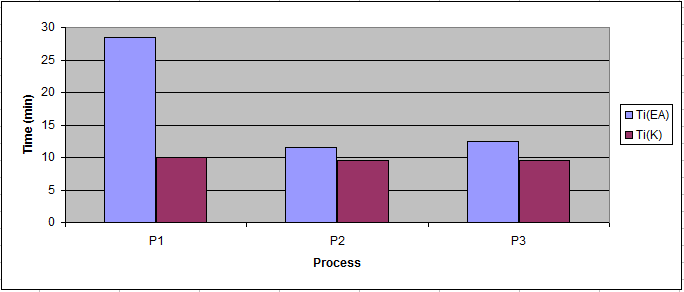
\includegraphics[scale=0.6 ,natwidth=682pt, natheight=290pt]{time.png}
	\caption{Promedios de Tiempo en la Tarea de An\'alisis 1}
	\label{fig:time}
\end{center}
\end{figure}

\begin{figure}[!t]
\begin{center}
	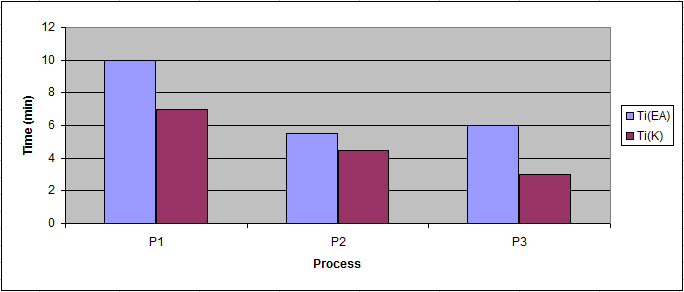
\includegraphics[scale=0.6 ,natwidth=682pt, natheight=291pt]{time2.png}
	\caption{Promedios de Tiempo en la Tarea de An\'alisis 2}
	\label{fig:time2}
\end{center}
\end{figure}

\begin{figure}[!t]
\begin{center}
	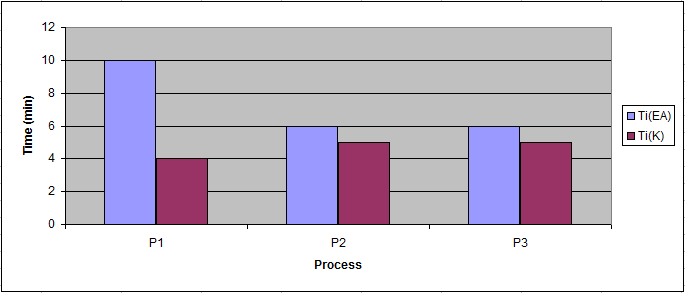
\includegraphics[scale=0.6 ,natwidth=684pt, natheight=292pt]{time3.png}
	\caption{Promedios de Tiempo en la Tarea de An\'alisis 3}
	\label{fig:time3}
\end{center}
\end{figure}

%........................................................

En la Figuras \ref{fig:results}, \ref{fig:results2} y \ref{fig:results3} se presenta el promedio de exactitud de todos los arquitectos realizando cada tareas sobre cada proceso. En cada Figura se compara para cada tarea (\texttt{T1, T2} y \texttt{T3}) la exactitud utilizando las herramientas tradicionales (\textit{EA}) y utilizando Kalcas \textit{K}.

%........................................................

\begin{figure}[!t]
\begin{center}
	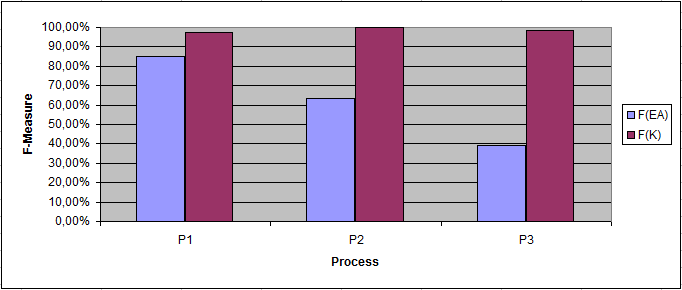
\includegraphics[scale=0.6 ,natwidth=682pt, natheight=289pt]{results.png}
	\caption{Promedios de Exactitud en la Tarea de An\'alisis 1}
	\label{fig:results}
\end{center}
\end{figure}

\begin{figure}[!t]
\begin{center}
	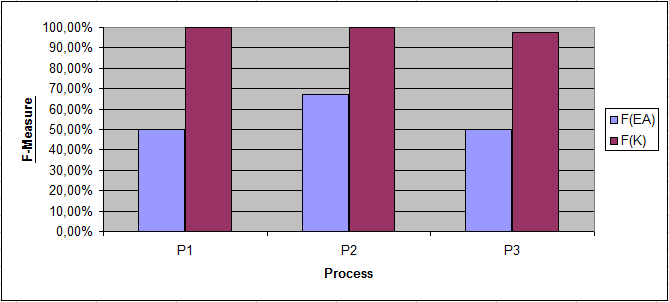
\includegraphics[scale=0.6 ,natwidth=669pt, natheight=302pt]{results2.png}
	\caption{Promedios de Exactitud en la Tarea de An\'alisis 2}
	\label{fig:results2}
\end{center}
\end{figure}

\begin{figure}[!t]
\begin{center}
	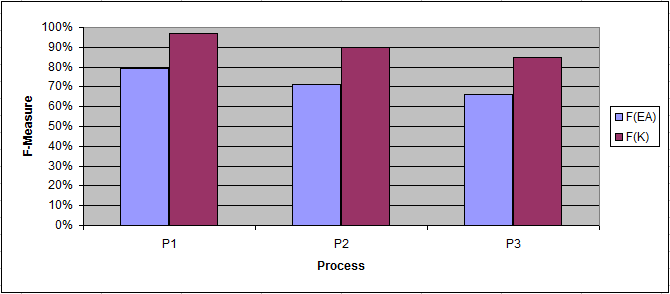
\includegraphics[scale=0.6 ,natwidth=669pt, natheight=293pt]{results3.png}
	\caption{Promedios de Exactitud en la Tarea de An\'alisis 3}
	\label{fig:results3}
\end{center}
\end{figure}

%........................................................

En general obtuvimos un aumento en la exactitud y por tanto una disminuci\'on de errores en las tareas de an\'alisis apoyadas en Kalcas. Particularmente, los mejores resultados en la tarea \texttt{T1} se obtuvo entre \texttt{P2-S2} y \texttt{P3-S3}, donde logramos aumentar la exactitud hasta en un 36\% y 59\% respectivamente. Tras analizar esta situaci\'on junto con los arquitectos, concluimos que la posible raz\'on es que el detalle del proceso \texttt{P1} es el m\'as conocido y socializado entre el grupo de arquitectos participantes, por tanto desde primera tarea de an\'alisis sin utilizar Kalcas ya se alcanz\'o un buen nivel de precisi\'on. Y por tanto Kalcas solo logr\'o refinarlo en un 11.9\%. Por otro lado, el detalle de los procesos \texttt{P2} y \texttt{P3} son menos conocidos por los arquitectos y de all\'i que Kalcas permiti\'o incrementar la exactitud en un 59\%. De manera similar la tarea \texttt{T2} al ser realizada utilizando Kalcas, present\'o mejoras entre el 32\% y el 50\% de exactitud. En cuanto a la tarea \texttt{T3} aunque tambi\'en present\'o mejoras fue la que evidenci\'o menores niveles de optimizaci\'on en el uso de Kalcas. Se alcanzaron incrementos entre un 17\% y 18.9\% de exactitud, siendo los procesos \texttt{P2} y \texttt{P3} los mas favorecidos (18.9\%).

Con los resultados obtenidos y volviendo sobre las hip\'otesis definidas en la Secci\'on \ref{sec:hypothesis} podemos concluir que la hip\'otesis H$_{11}$ es aceptada en cuanto el valor F-Measure fue menor para todos los casos soportados con Kalcas: H$_{10}$ - Rejected; H$_{11}$ - Accepted. La hip\'otesis H$_{21}$ es aceptada en cuanto el tiempo al realizar las tareas de an\'alisis fue menor cuando se apoyaron en Kalcas: H$_{20}$ - Rejected; H$_{21}$ - Accepted.

Con las tareas \texttt{T2} y \texttt{T3} pudimos expresar y evaluar las heur\'isticas descritas en el Cap\'itulo \ref{cha:intro}. Los resultados de evaluar los procesos y esquemas del ICFES con estas heur\'isticas se presentan en la Tabla \ref{tab:alignmentAB}.

\begin{table}
\begin{center}
\scalebox{1}{
\begin{tabular}{c c c} \hline
Heur\'istica Evaluada & Conjuntos Comparados & Hallazgos\\
\hline
Actividades que no acceden a ninguna entidad & P1-S1 & - \\
Actividades que no acceden a ninguna entidad & P2-S2 & 6 \\
Actividades que no acceden a ninguna entidad & P3-S3 & 6 \\
Entidades no accedidas por ninguna actividad & P1-S1 & 2 \\
Entidades no accedidas por ninguna actividad & P2-S2 & 1 \\
Entidades no accedidas por ninguna actividad & P3-S3 & 1 \\
Entidades redundantes & S1-S2 & 11	\\
Entidades redundantes & S1-S3 & 6 \\
Entidades redundantes & S2-S3 & 6 \\
Actividades redundantes & P1-P2 & 8 \\
Actividades redundantes & P1-P3 & 3 \\
Actividades redundantes & P2-P3 & 5 \\
\hline
\end{tabular}
}
\end{center}
\caption{Resultados de Evaluar Heur\'isticas de Desalineaci\'on}
\label{tab:alignmentAB}
\end{table}

Luego del an\'alisis de estos resultados, encontramos que los componentes redundantes detectados corresponden a procesos o entidades solapadas, dado que los dos procesos analizados son an\'alogos o por lo menos conceptualmente similares y por tanto tienen actividades y entidades en com\'un. La redundancia tanto de procesos como de entidades no implica un problema como tal, dado que bajo algunos escenarios la redundancia es conocida y hasta justificada, pero es importante identificar y evaluar dichos solapamientos. Los casos de objetos desalineados fueron analizados con mayor profundidad y llegamos a algunas conclusiones que ser\'an presentadas mas adelante en el Cap\'itulo \ref{cha:conclusions}.

Tras esta experimentaci\'on realizamos entrevistas con los arquitectos para recoger impresiones y aportes con respecto al uso de Kalcas, esto con el fin de retroalimentar esta propuesta desde un punto de vista mas cercano a la industria. Como ventajas, los usuarios resaltaron la agilidad y precisi\'on con la que Kalcas apoyaba sus an\'alsis sobre BA e IA. Tambi\'en fueron destacadas las opciones del editor para manejar a diferentes niveles de granularidad dentro de cada dominio, dado que se pod\'ian analizar procesos o esquemas completos o centrarse en entidades y actividades particulares. Como puntos a mejorar se recalc\'o la poca fluidez en los pasos para desplegar las herramientas y ejecutar las consultas. Esto debido a que las opciones para importar las arquitecturas, desplegar el editor KQL y ejecutar las consultas requer\'ian la configuraci\'on de archivos de propiedades, ejecuci\'on de instancias de eclipse y algunos pasos adicionales dentro del IDE para obtener los reportes de salida. Tenemos claro que la actual implementaci\'on requiere mas trabajo de integraci\'on y desarrollo de GUI para lograr ser utilizada adecuadamente en un entorno industrial. Otra posibilidad de mejora consiste en la legibilidad del reporte cuando se entra a analizar procesos o esquemas con gran cantidad de elementos, debido a que los diagramas de grafos generados en formato PNG por el algoritmo de Graphviz se tornan mas complejos y dif\'iciles de entender. En este punto se presentaron sugerencias como la exploraci\'on de reportes din\'amicos, que permitan navegar sobre el grafo, seleccionar y resaltar trazas de manera que se facilite la identificaci\'on de relaciones entre los conceptos. Para afrontar el problema de la complejidad, los arquitectos utilizaron la opci\'on de focalizar las consultas sobre determinadas entidades o actividades que eran objeto de an\'alisis. 

Finalmente, para el momento del experimento se hab\'ia llevando a cabo dentro del Instituto un proceso de mapear los procesos de negocio con las entidades, el cual fue costoso de realizar dado que tales relaciones no estaban formalizadas, sino en la mente de los arquitectos y analistas que participan en dichos procesos, y es all\'i donde la organizaci\'on vi\'o una oportunidad para obtener importantes aportes en la ejecuci\'on de tales tareas de alineamiento. Sumado a esto, la identificaci\'on de redundancias y desalineaciones sobre BA e IA le brind\'o un valor agregado al Instituto. En algunos casos para evidenciar algunos solapamientos que aunque no eran desconocidos, tampoco estaban formalmente identificados. En otros casos el experimento logr\'o identificar oportunidades en cuanto a mejorar la alineaci\'on en algunos componentes puntuales de la EA.